% Chapter 7

\chapter{Benchmarking}
\label{Chapter7}

In this chapter we present several metrics that can be used to evaluate the performance of the transfer learning techniques that we presented in Chapter~\ref{Chapter6}.

We also report the results on our reinforcement learning domain following such metrics.

These metrics are important to critically evaluate and compare these techniques with baseline models.

% Baseline:
% Vanilla Q-learning
% Q-learning with L2 (towards zero) regularisation
% Q-learning with L2 (towards average of source tasks, conventional transfer learning) regularisation

% Metrics:
% Timestamp of acceptable reward
% AuC


\section{Metrics and baseline model}
\label{sec:metricsbaselinemodel}
One first step necessary to evaluate success in the resolution of reinforcement learning tasks is to plot the rewards over time, and verifying the asymptotic trend of the curve.

Usually these will converge to a certain value, which is indicative of the performance of the models that we trained. The approach that OpenAI takes in evaluating success of certain policy that has been trained is to set a fixed reward threshold above which the task is considered solved. For example, the vanilla \code{FrozenLake-v0} implementation with the fixed map configuration we showed in figure~\ref{tab:FrozenLakev0}, is considered "solved" if the policy achieves an average reward of 0.78 over 100 consecutive trials.

While our implementation of \code{RandomisedFrozenLake} directly builds on the \code{FrozenLake-v0} environment, using the same average reward threshold for our set up will not work. The reason being that the map configuration of \code{FrozenLake-v0} has a fixed degree of difficulty indicated by the number of holes in the map. The threshold of 0.78 directly has been set given this difficulty.
\code{RandomisedFrozenLake} environments have a varying amount of holes and, as a consequence, of difficulty. To set our threshold, we plot in figure~\ref{fig:QlearningBaselineBench} the average rewards achieved by the Q-tables in the test set while training with vanilla Q-learning. Each timestep corresponds to the average reward achieved with the 765 policies in the test set at the corresponding timestep. We also plot the standard deviations (dashed blue lines) of these rewards. Furthermore, to plot this curve we take the rolling window average of 20 timesteps to avoid wildly oscillating reward curves.

We notice right away that in fact we never even reach a value of 0.78 in our average rewards. That is because map configurations in the test set contain tasks that are on average harder (i.e. contain more holes) than \code{FrozenLake-v0}.

The test policies rewards asymptotically converge to 0.36, which may seem low compared to \code{FrozenLake-v0}'s 0.78, but it is once again taken as an average of all maps in the test set. That also justifies the wide standard deviations on the plot, as it virtually ranges the whole reward boundaries $(0,1)$.

Given this analysis, we set the average threshold reward value to 0.32 (grey dashed/dotted line), which vanilla Q-learning reaches after around 250,000 training timesteps.

\begin{figure}[H]
\centering
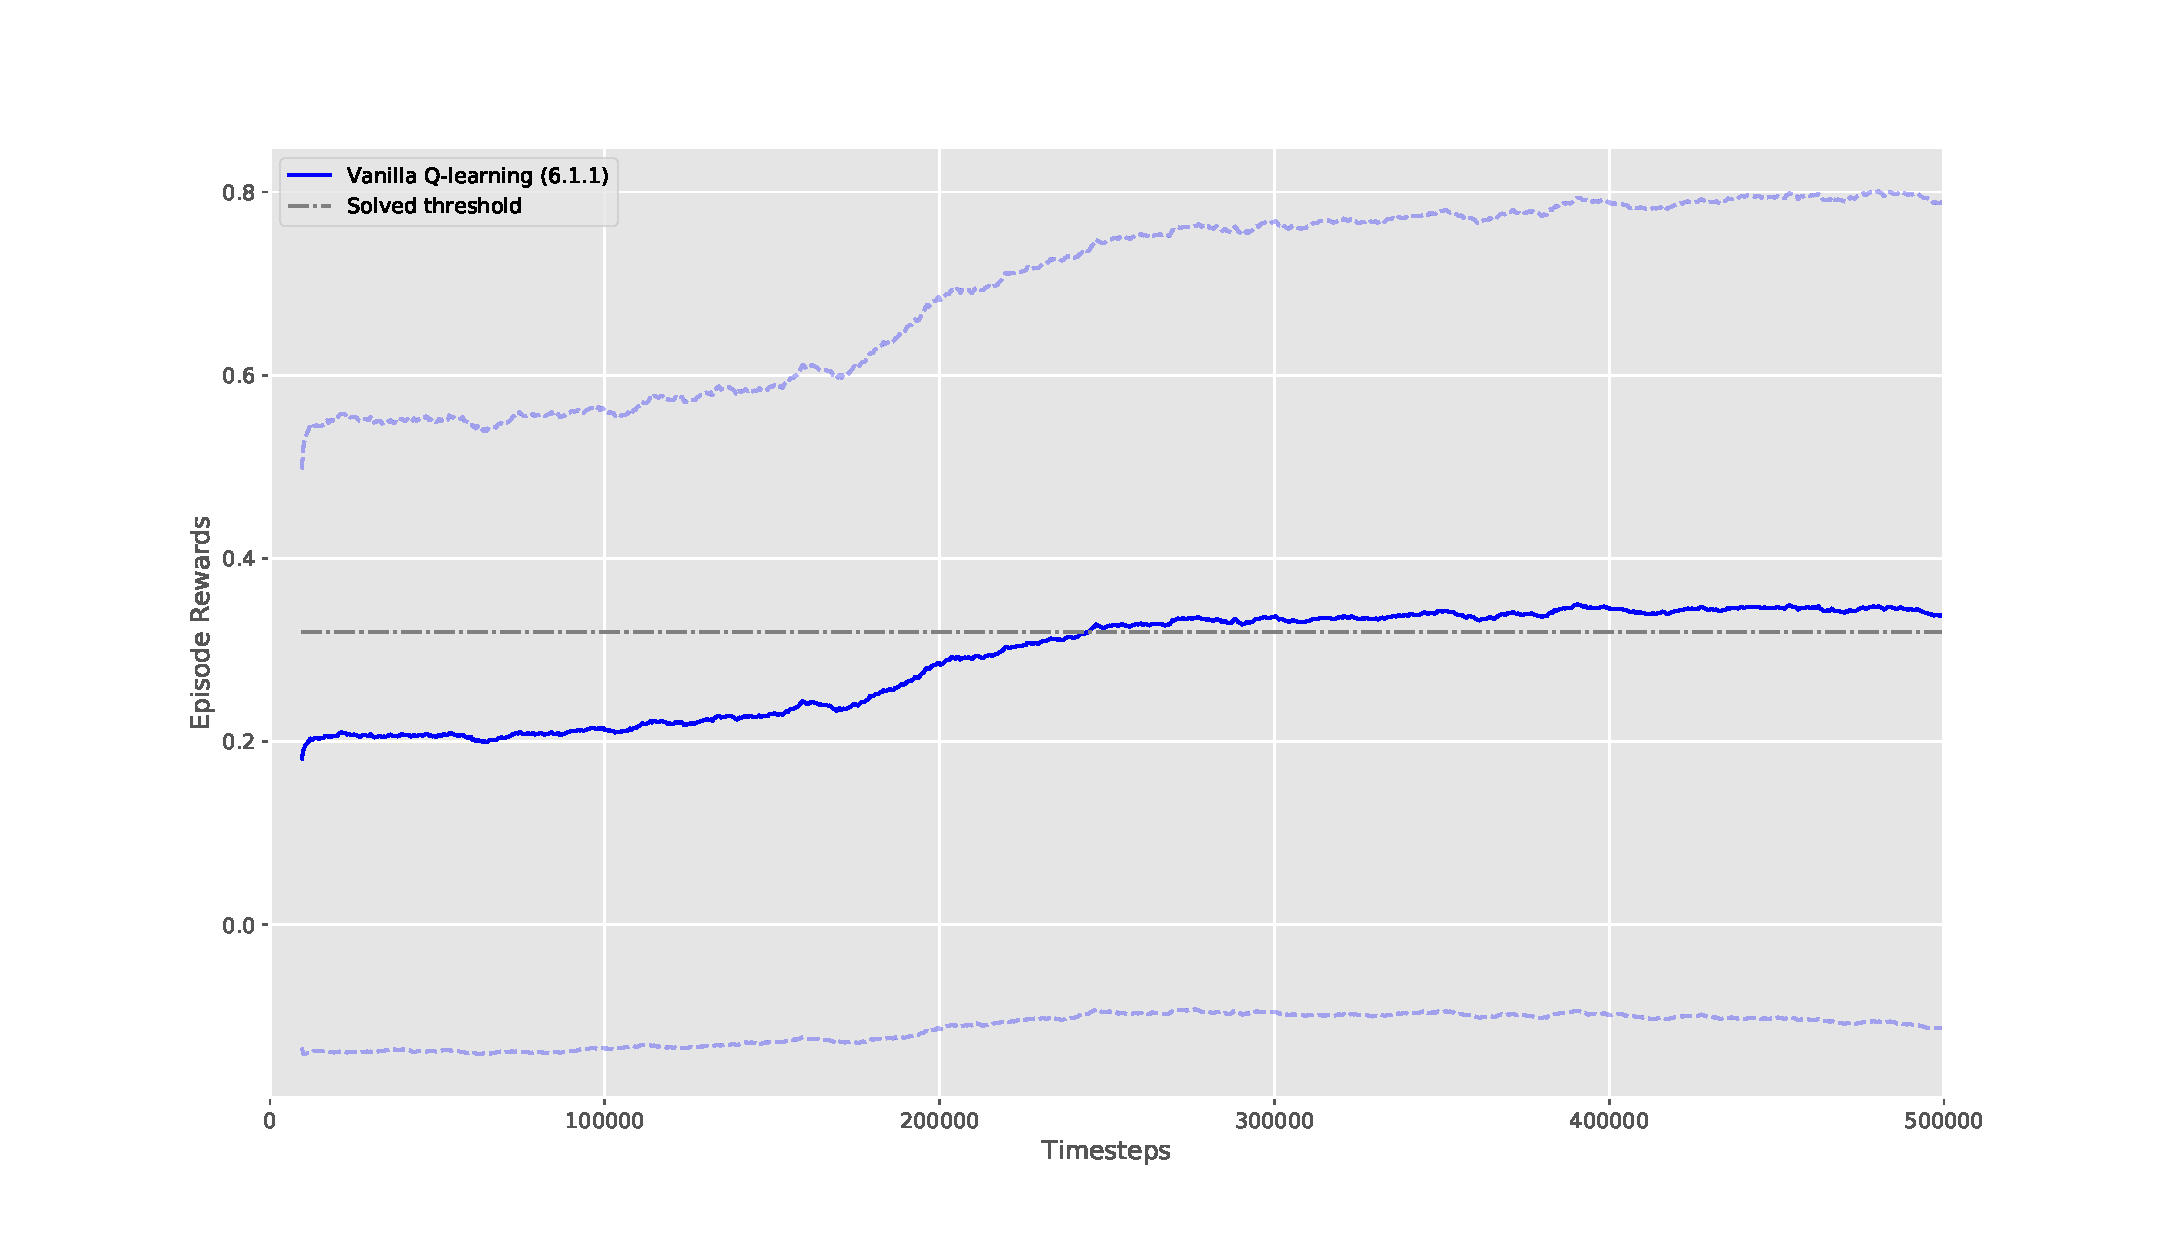
\includegraphics[width=15cm]{Figures/QlearningBaselineBench}
\caption{Vanilla Q-learning: Rewards over timesteps}
\label{fig:QlearningBaselineBench}
\end{figure}


\section{Discriminator techniques}


\subsection{Update whole Q-table (Approach \ref{ssec:QlearningGANWhole})}
Figure~\ref{fig:QlearningGANWholeBench} shows the results of the model that we presented in section 6.1.2, which updates the whole Q-table after each timestep (magenta plot). 
We also include both baselines: the model trained with vanilla Q-learning (blue) and the model that uses L2 regularisation towards the average of the training Q-tables (orange).
As usual, we plot the standard deviations of all models.
We notice how vanilla Q-learning performs better than these two models that use transfer learning.
We motivate this poor performance on the fact that update the whole Q-table can throw off vanilla Q-learning and the $\epsilon$-greedy approach fails to recover after each inaccurate update towards the gradient of the discriminator.

Our method, while being less efficient than Q-learning in terms of the average rewards obtained on the test domains, nevertheless manages to solve the domain after an average of 430,000 timesteps, which is still much higher than the 250,000 timesteps of vanilla Q-learning.

\begin{figure}[H]
\centering
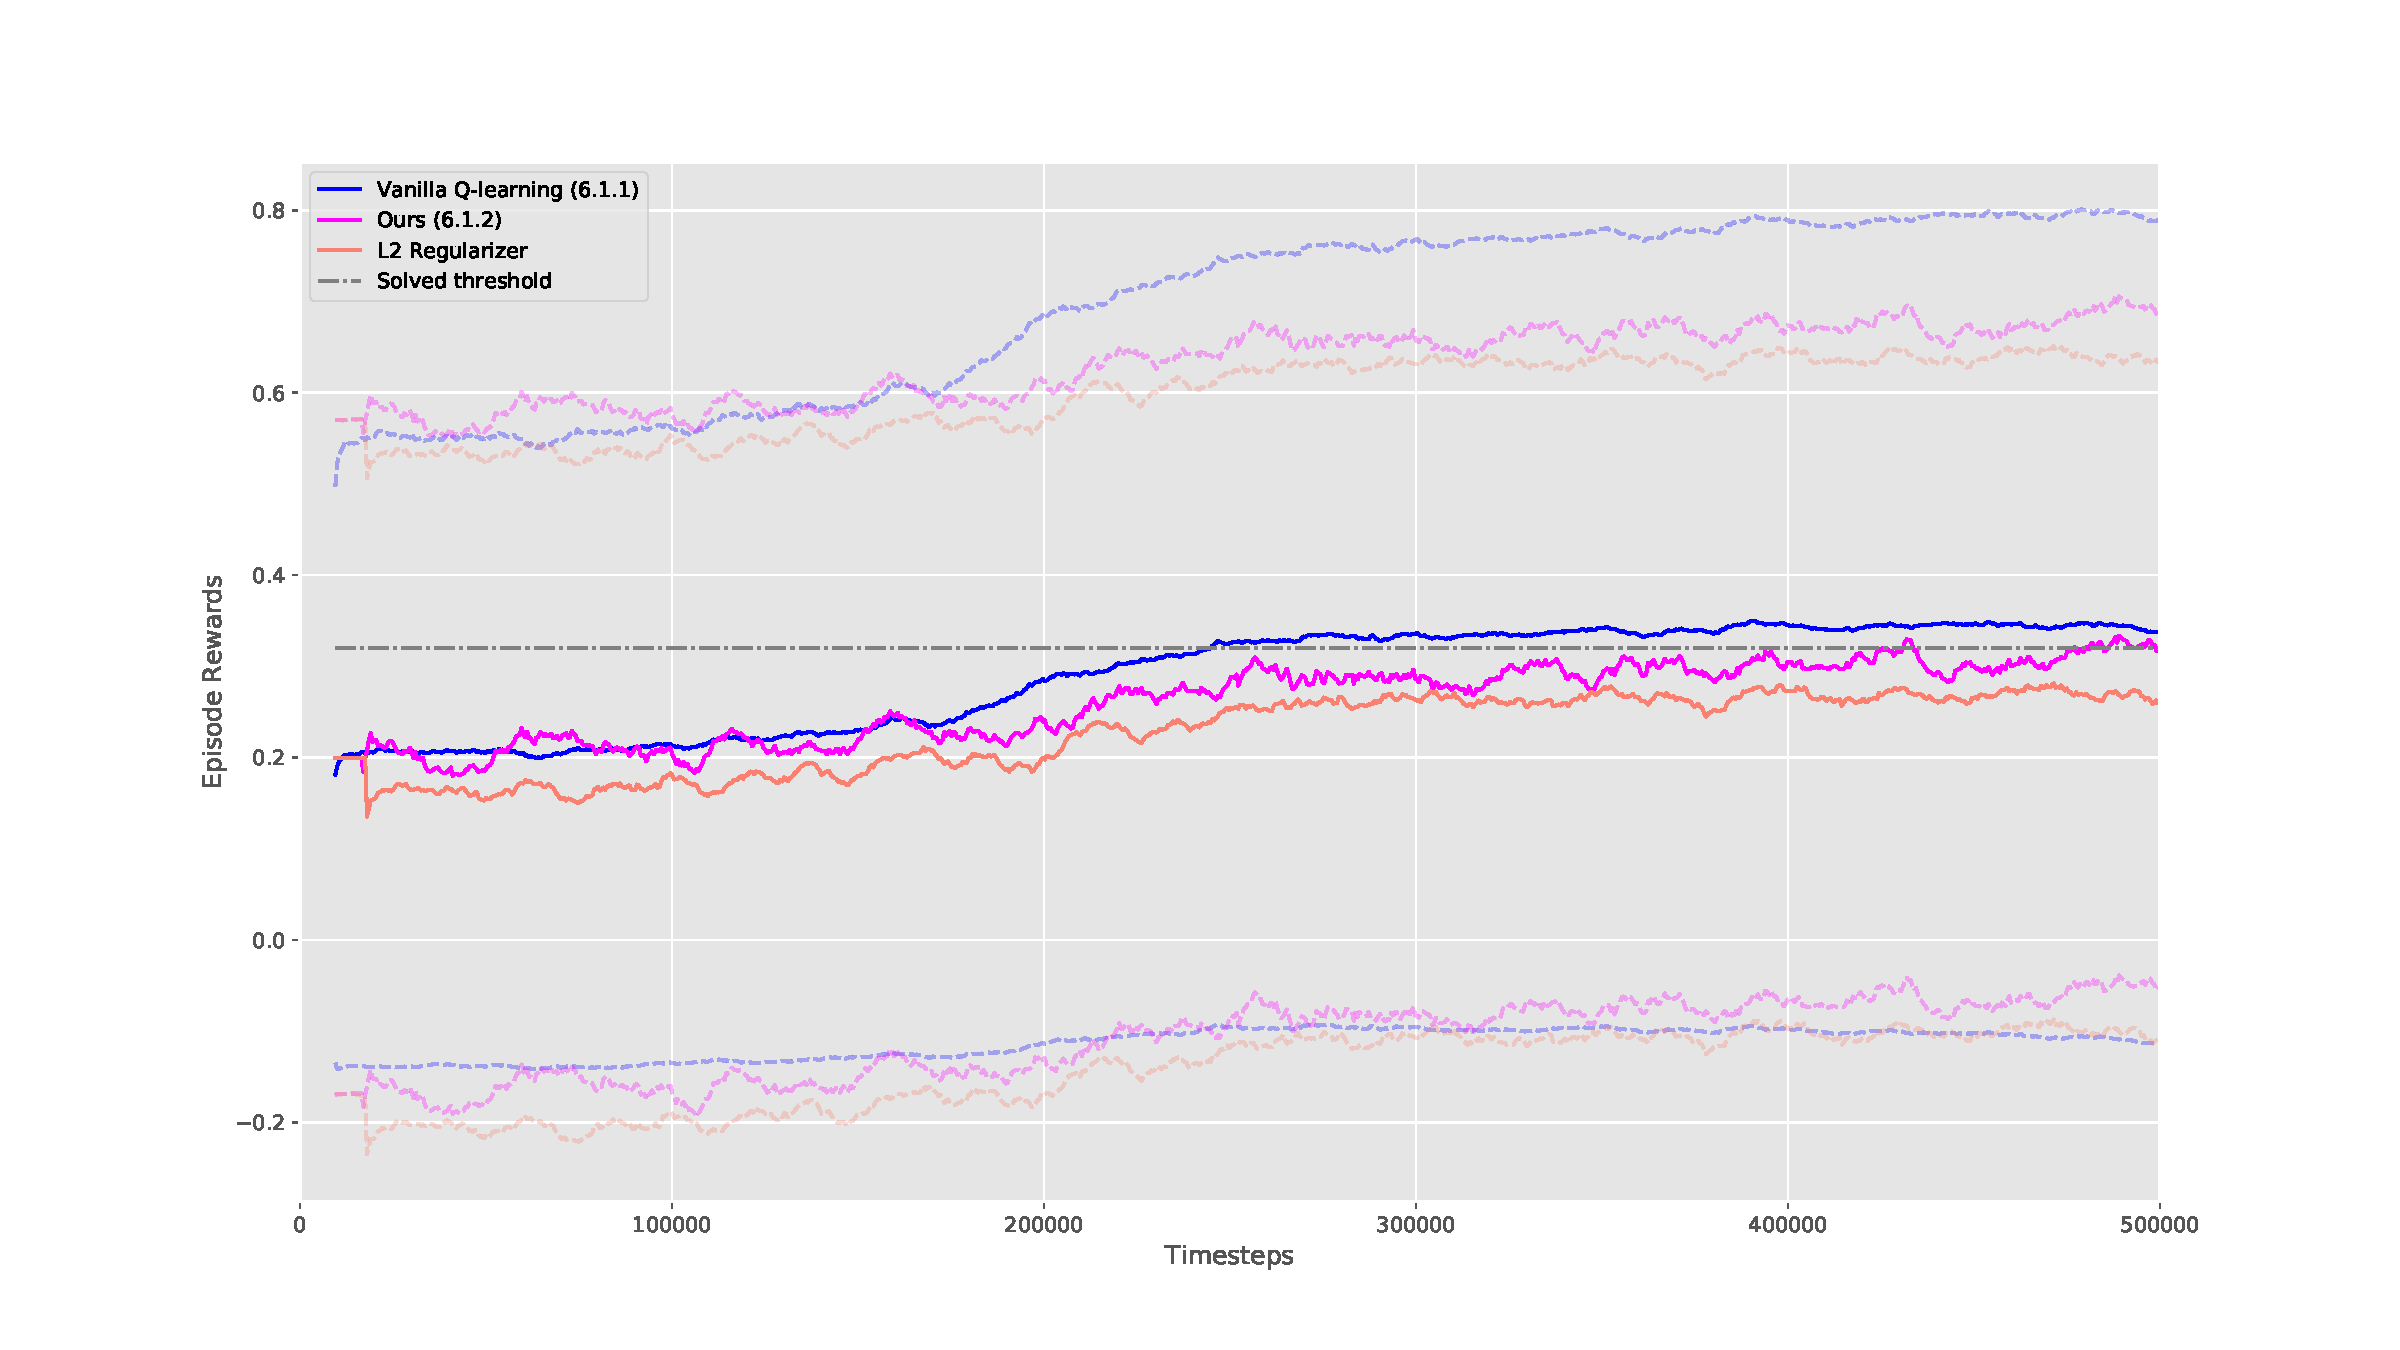
\includegraphics[width=15cm]{Figures/QlearningGANWholeBench}
\caption{Q-learning with whole Q-table: Rewards over timesteps}
\label{fig:QlearningGANWholeBench}
\end{figure}


\subsection{Update Q-table pair (Approach \ref{ssec:QlearningGANPair})}
Figure~\ref{fig:QlearningGANPairBench} shows the results of the transfer learning approach whereby instead of updating the whole Q-table towards the direction of $\nabla D(Q_{t})$, we update only the state/action pair in that particular timestep.

\begin{figure}[H]
\centering
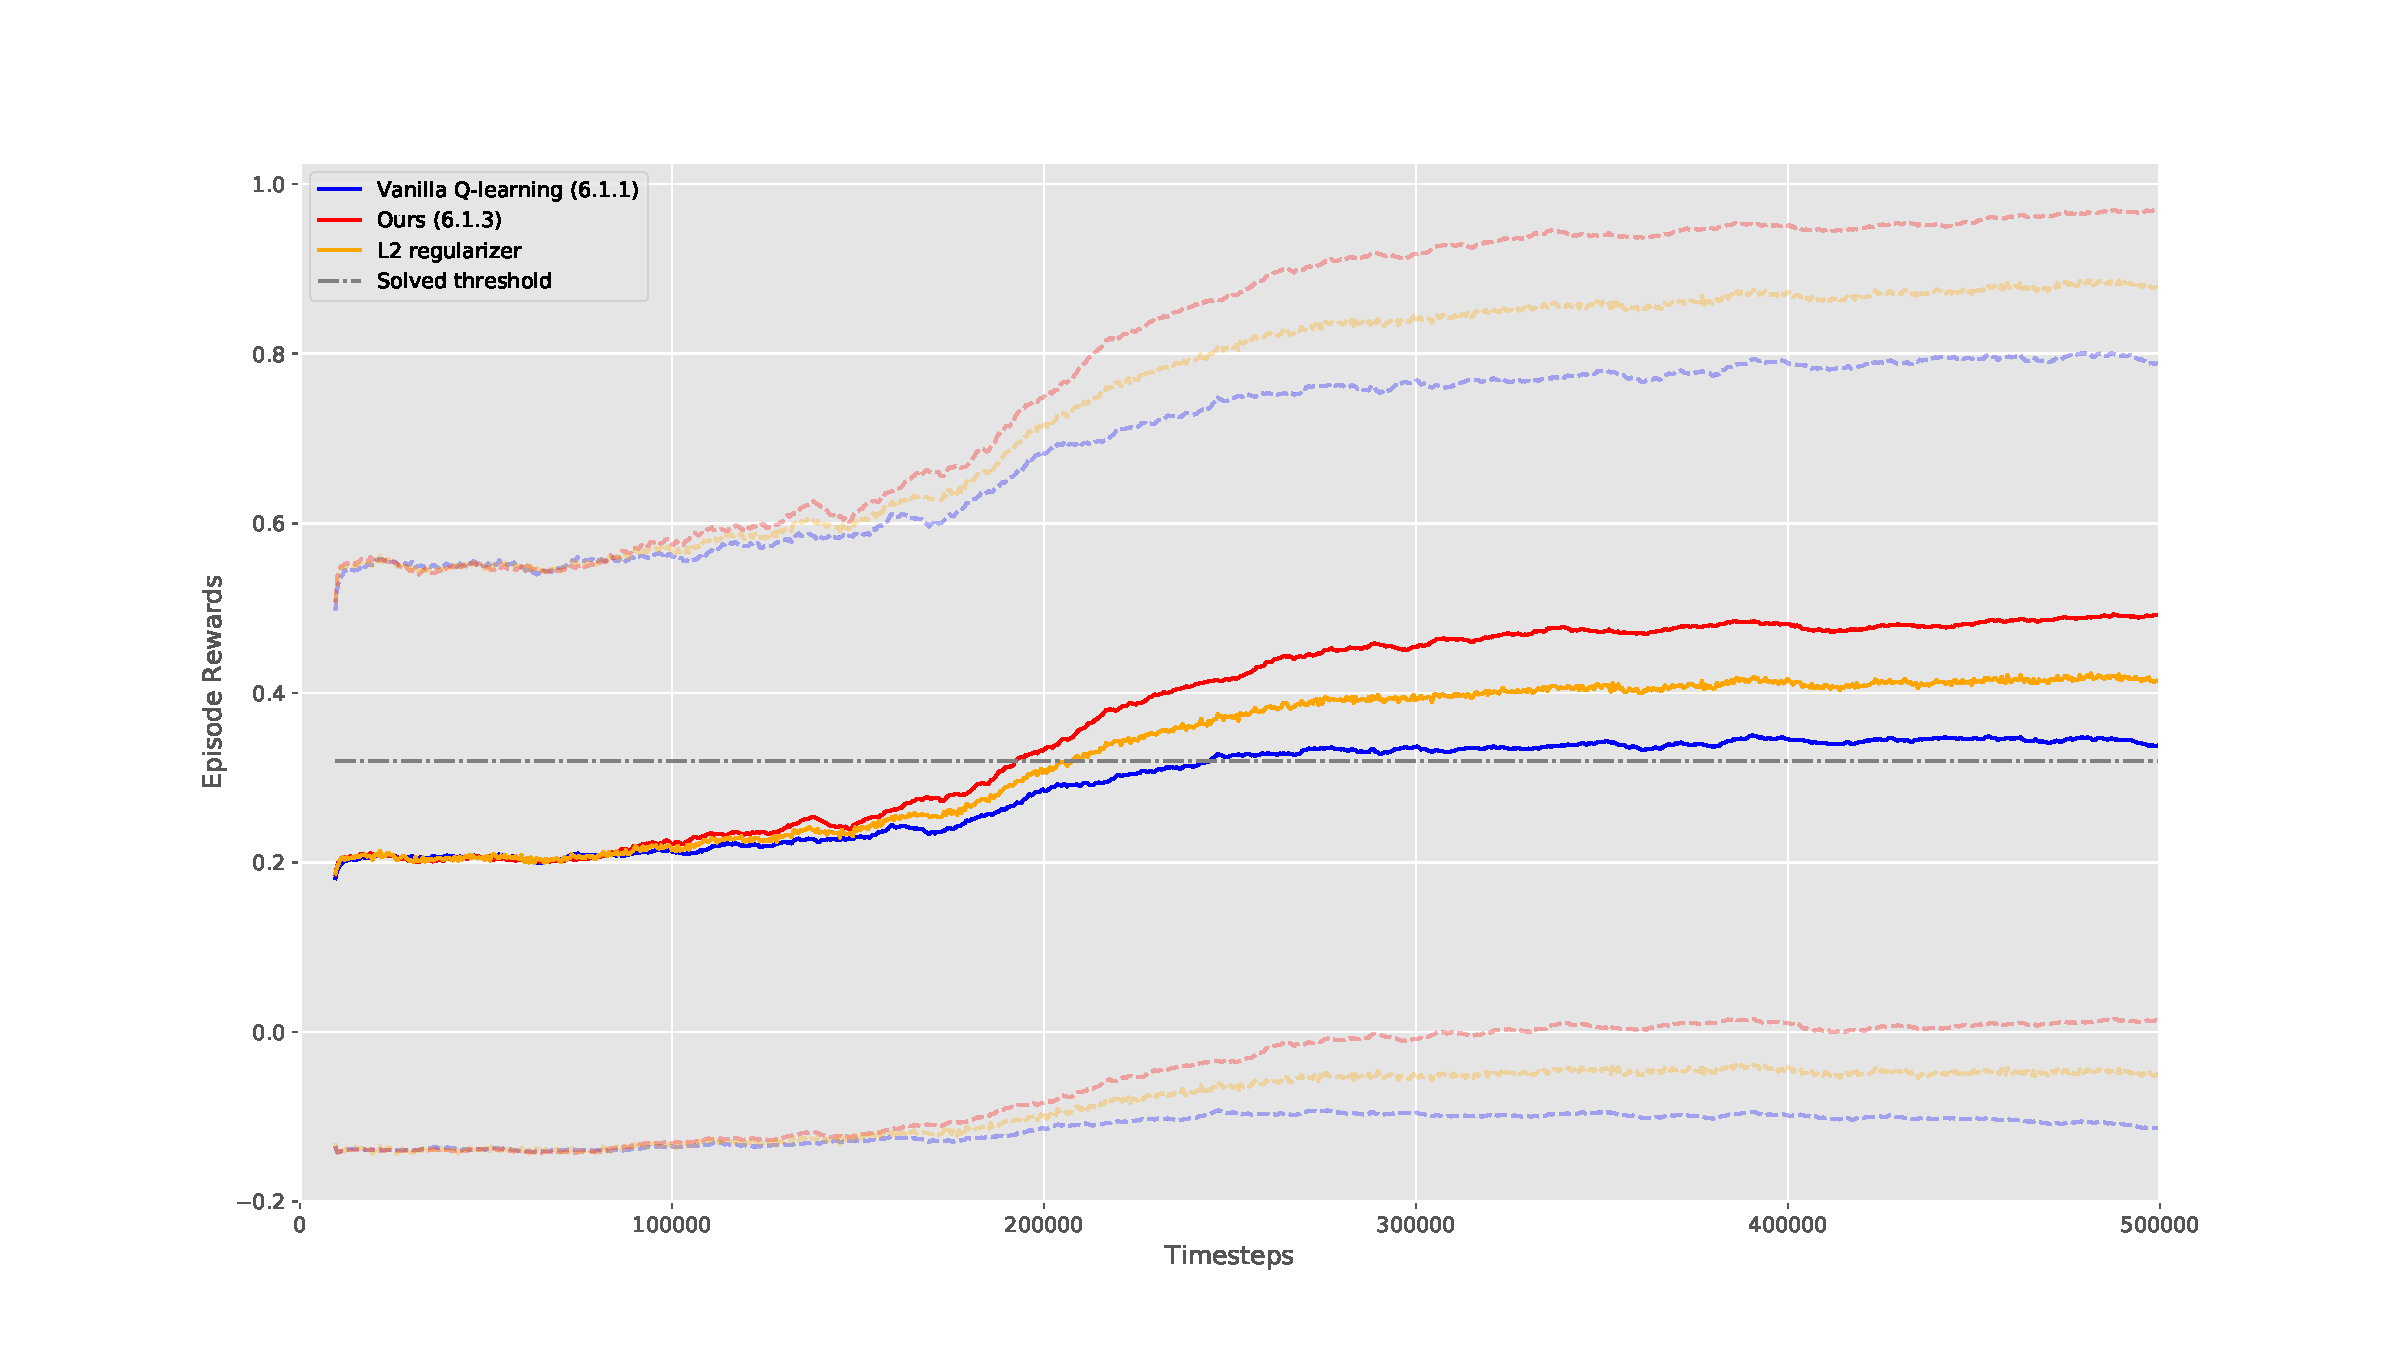
\includegraphics[width=15cm]{Figures/QlearningGANPairBench}
\caption{Q-learning with state/action pair update: Rewards over timesteps}
\label{fig:QlearningGANPairBench}
\end{figure}

We see right away that our model (red plot) asymptotically achieves much higher average rewards than our baseline models. We solve the task at just over 190,000 timesteps by reaching our reward threshold  of 0.32 much earlier than our baseline models.

Just like in the previous benchmark, here we also take into account the model with L2 regularisation towards the mean of the test set as one of our baseline. However, instead of again updating the whole table, we update the corresponding state/action value in the Q-table. We see that while that performs better than vanilla Q-learning, the discriminative model trained with the GAN is better able to capture transferrable information to feed back to the iterative Q-table update. 


\subsection{Update Q-table row (Approach \ref{ssec:QlearningGANRow})}
This approach is not as conservative as the previous one, as it updates the whole row of the state the agent is in after each timestep.

This model also performs better than both baselines, solving the task after an average of 210,000 timesteps.

Once again, the L2 regulariser baseline only pushes the appropriate row towards the mean Q-tables, rather than the whole table.

\begin{figure}[H]
\centering
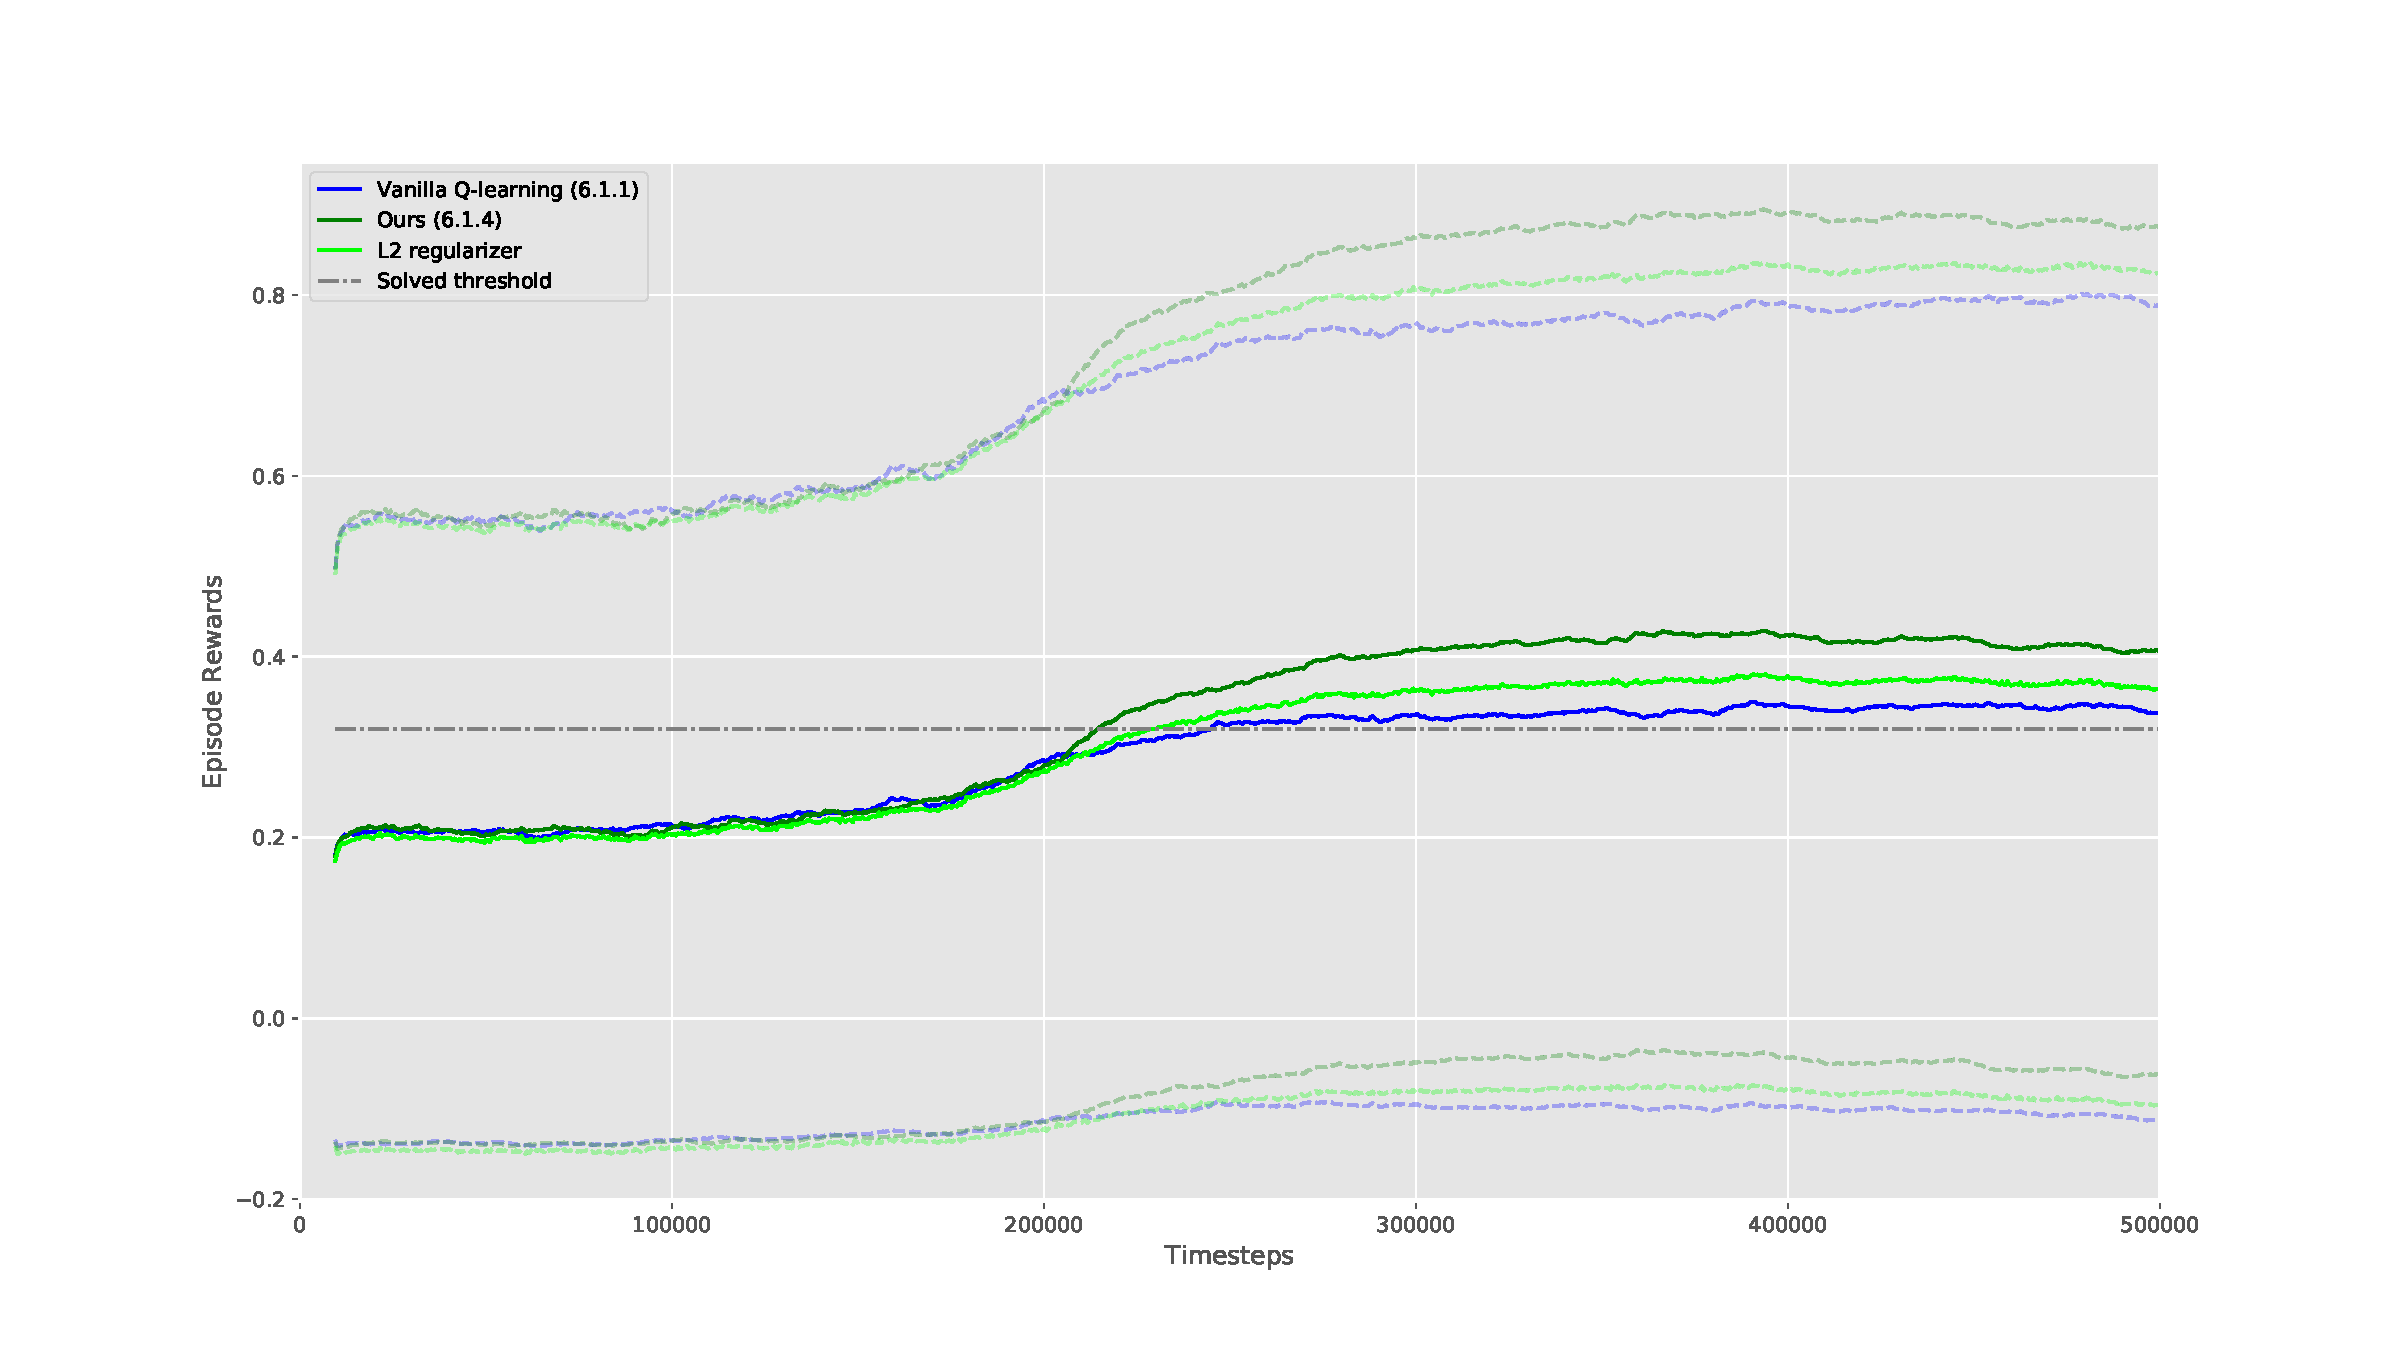
\includegraphics[width=15cm]{Figures/QlearningGANRowBench}
\caption{Q-learning with row update: Rewards over timesteps}
\label{fig:QlearningGANRowBench}
\end{figure}

\subsection{Discriminator benchmarks overview}
Here in figure~\ref{fig:QlearningGANAllDiscrim} we display the overall results of our transfer learning techniques compared to the vanilla Q-learning results. Table~\ref{tab:aucdiscrim} reports in descending order the area under the curve metric (AuC) of each average reward plot. We can use this metric to measure the overall cumulative rewards during training. In combination with the reward threshold line, we can have through these two metrics a summative overview of how our models are performing when transferring knowledge.

\begin{figure}[H]
\centering
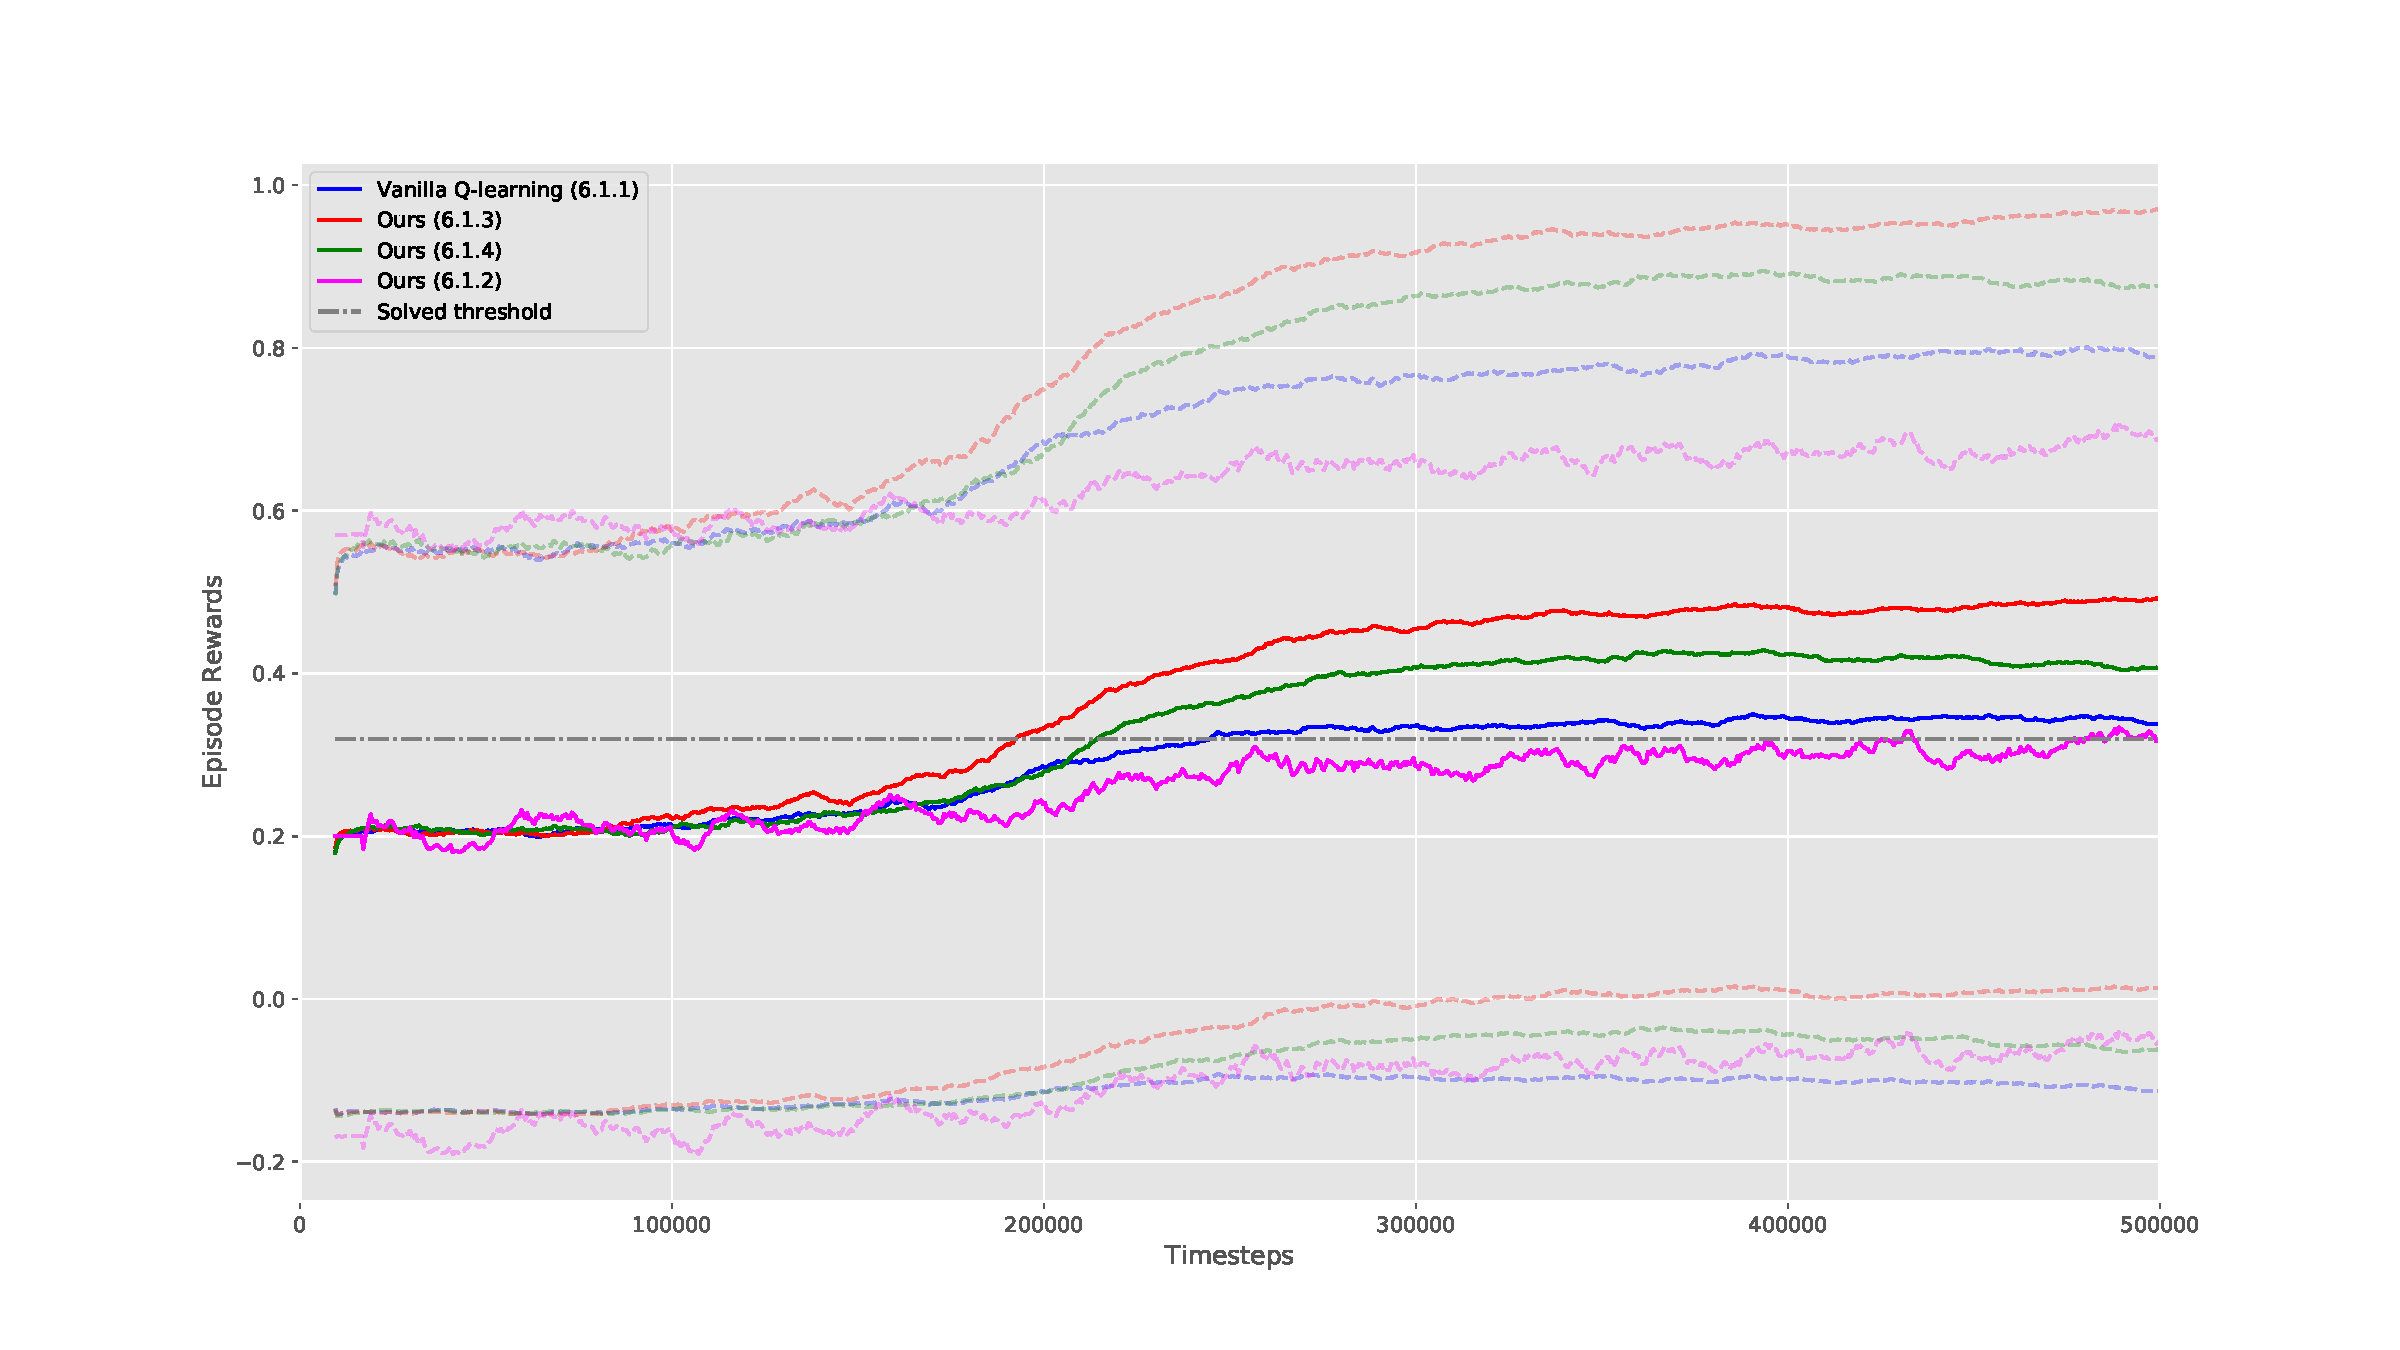
\includegraphics[width=15cm]{Figures/QlearningGANAllDiscrim}
\caption{Q-learning with state/action pair update: Rewards over timesteps}
\label{fig:QlearningGANAllDiscrim}
\end{figure}


\begin{table}[H]
\centering
\begin{tabular}{@{}ll@{}}
\toprule
Transfer learning approach & AuC     \\ \midrule
Q-table state/pair update (approach~\ref{ssec:QlearningGANPair})  & 1816.29 \\
Q-table row update (approach~\ref{ssec:QlearningGANRow})        & 1615.63 \\
Vanilla GAN (baseline)     & 1420.80 \\
Whole Q-table update (approach~\ref{ssec:QlearningGANWhole})      & 1282.46 \\ \bottomrule
\end{tabular}
\caption{Area under the curve of different approaches in descending order of AuC}
\label{tab:aucdiscrim}
\end{table}

\section{Generator techniques}
\subsection{Global search (approach~\ref{ssec:globalsearch})}
With the global search technique, we directly sample Q-tables from the generator to use as policies for the task at hand. Thus, there is no direct training process in the sense of iterative Q-table updates.

The only fixed hyperparameter in this approach is the number of sampled Q-tables from the Generator network, from which we will pick the one that yields the best results in terms of rewards. This number great affects the runtime of the algorithm, as we need to check the rewards for each policy.

To find a good compromise between number of sampled policies and its performance on the test set, we build table~\ref{tab:avgrewardsglobalsearch}.

It is clear from this, that even by sample 100,000 policies, on average, the best policies do not perform as well as the baseline policies trained with vanilla Q-learning, which, as we saw in section~\ref{sec:metricsbaselinemodel} achieved an asymptotic average reward of 0.36, much more than the maximum of 0.2932 we achieve with global search.

It is still worth to reiterate that global search may still return good policies with domains that have a relatively small policy space.

\begin{table}[H]
\centering
\begin{tabular}{@{}ll@{}}
\toprule
\# sampled Q-tables/policies & Avg rewards test set \\ \midrule
1                            & 0.2123               \\
10                           & 0.2738               \\
1,000                        & 0.2801               \\
5,000                        & 0.2832               \\
10,000                       & 0.2902               \\
100,000                      & 0.2932               \\ \bottomrule
\end{tabular}
\caption{Average rewards in test set tasks for different number of sampled Q-tables/policies from the Generator}
\label{tab:avgrewardsglobalsearch}
\end{table}

\subsection{Global/local search (approach~\ref{ssec:localglobalsearch})}
The global/local search hybrid approach, we take in the best Q-table/policy found with global search, and use that Q-table as the starting point of our training.  We could use any technique from the previous section for local search, but to greatly limit the number of experiments that we need to run, we pick the model that performed best in our discriminator benchmarks earlier. That is approach~\ref{ssec:QlearningGANPair} where we update a single state/action pair from $\nabla D(Q_{t})$.

Table~\ref{tab:avgrewardslocalglobalsearch} shows the asymptotic performance after local search of each model when taking increasing number of sampled policies.

\begin{table}[H]
\centering
\begin{tabular}{@{}ll@{}}
\toprule
\# sampled Q-tables/policies & Avg rewards test set \\ \midrule
1                            & 0.5223               \\
10                           & 0.5238               \\
1,000                        & 0.5401               \\
5,000                        & 0.5632               \\
10,000                       & 0.5702               \\
100,000                      & 0.5712               \\ \bottomrule
\end{tabular}
\caption{Average rewards in test set tasks for different number of sampled Q-tables/policies from the Generator}
\label{tab:avgrewardslocalglobalsearch}
\end{table}

An optimal number of policies to sample seems to 10,000 for our environment setup, but it may vary for different domains and the result generally depends, particularly at lower number of sample Q-tables, on how fortuitous we are with the Q-tables that we sample from the Generator network.

Finally, figure~\ref{fig:globallocalsearchBench} shows the plot of the model when we take 10,000 sampled policies during local search. From this figure we notice a few things:
\begin{enumerate}
	\item The global/local search policy reaches the reward threshold earlier than our best model before.
	\item The overall rewards (i.e. AuC) will also be slightly better.
	\item The starting point derived from global search allows us to have better rewards even at earlier timesteps.
\end{enumerate}

\begin{figure}[H]
\centering
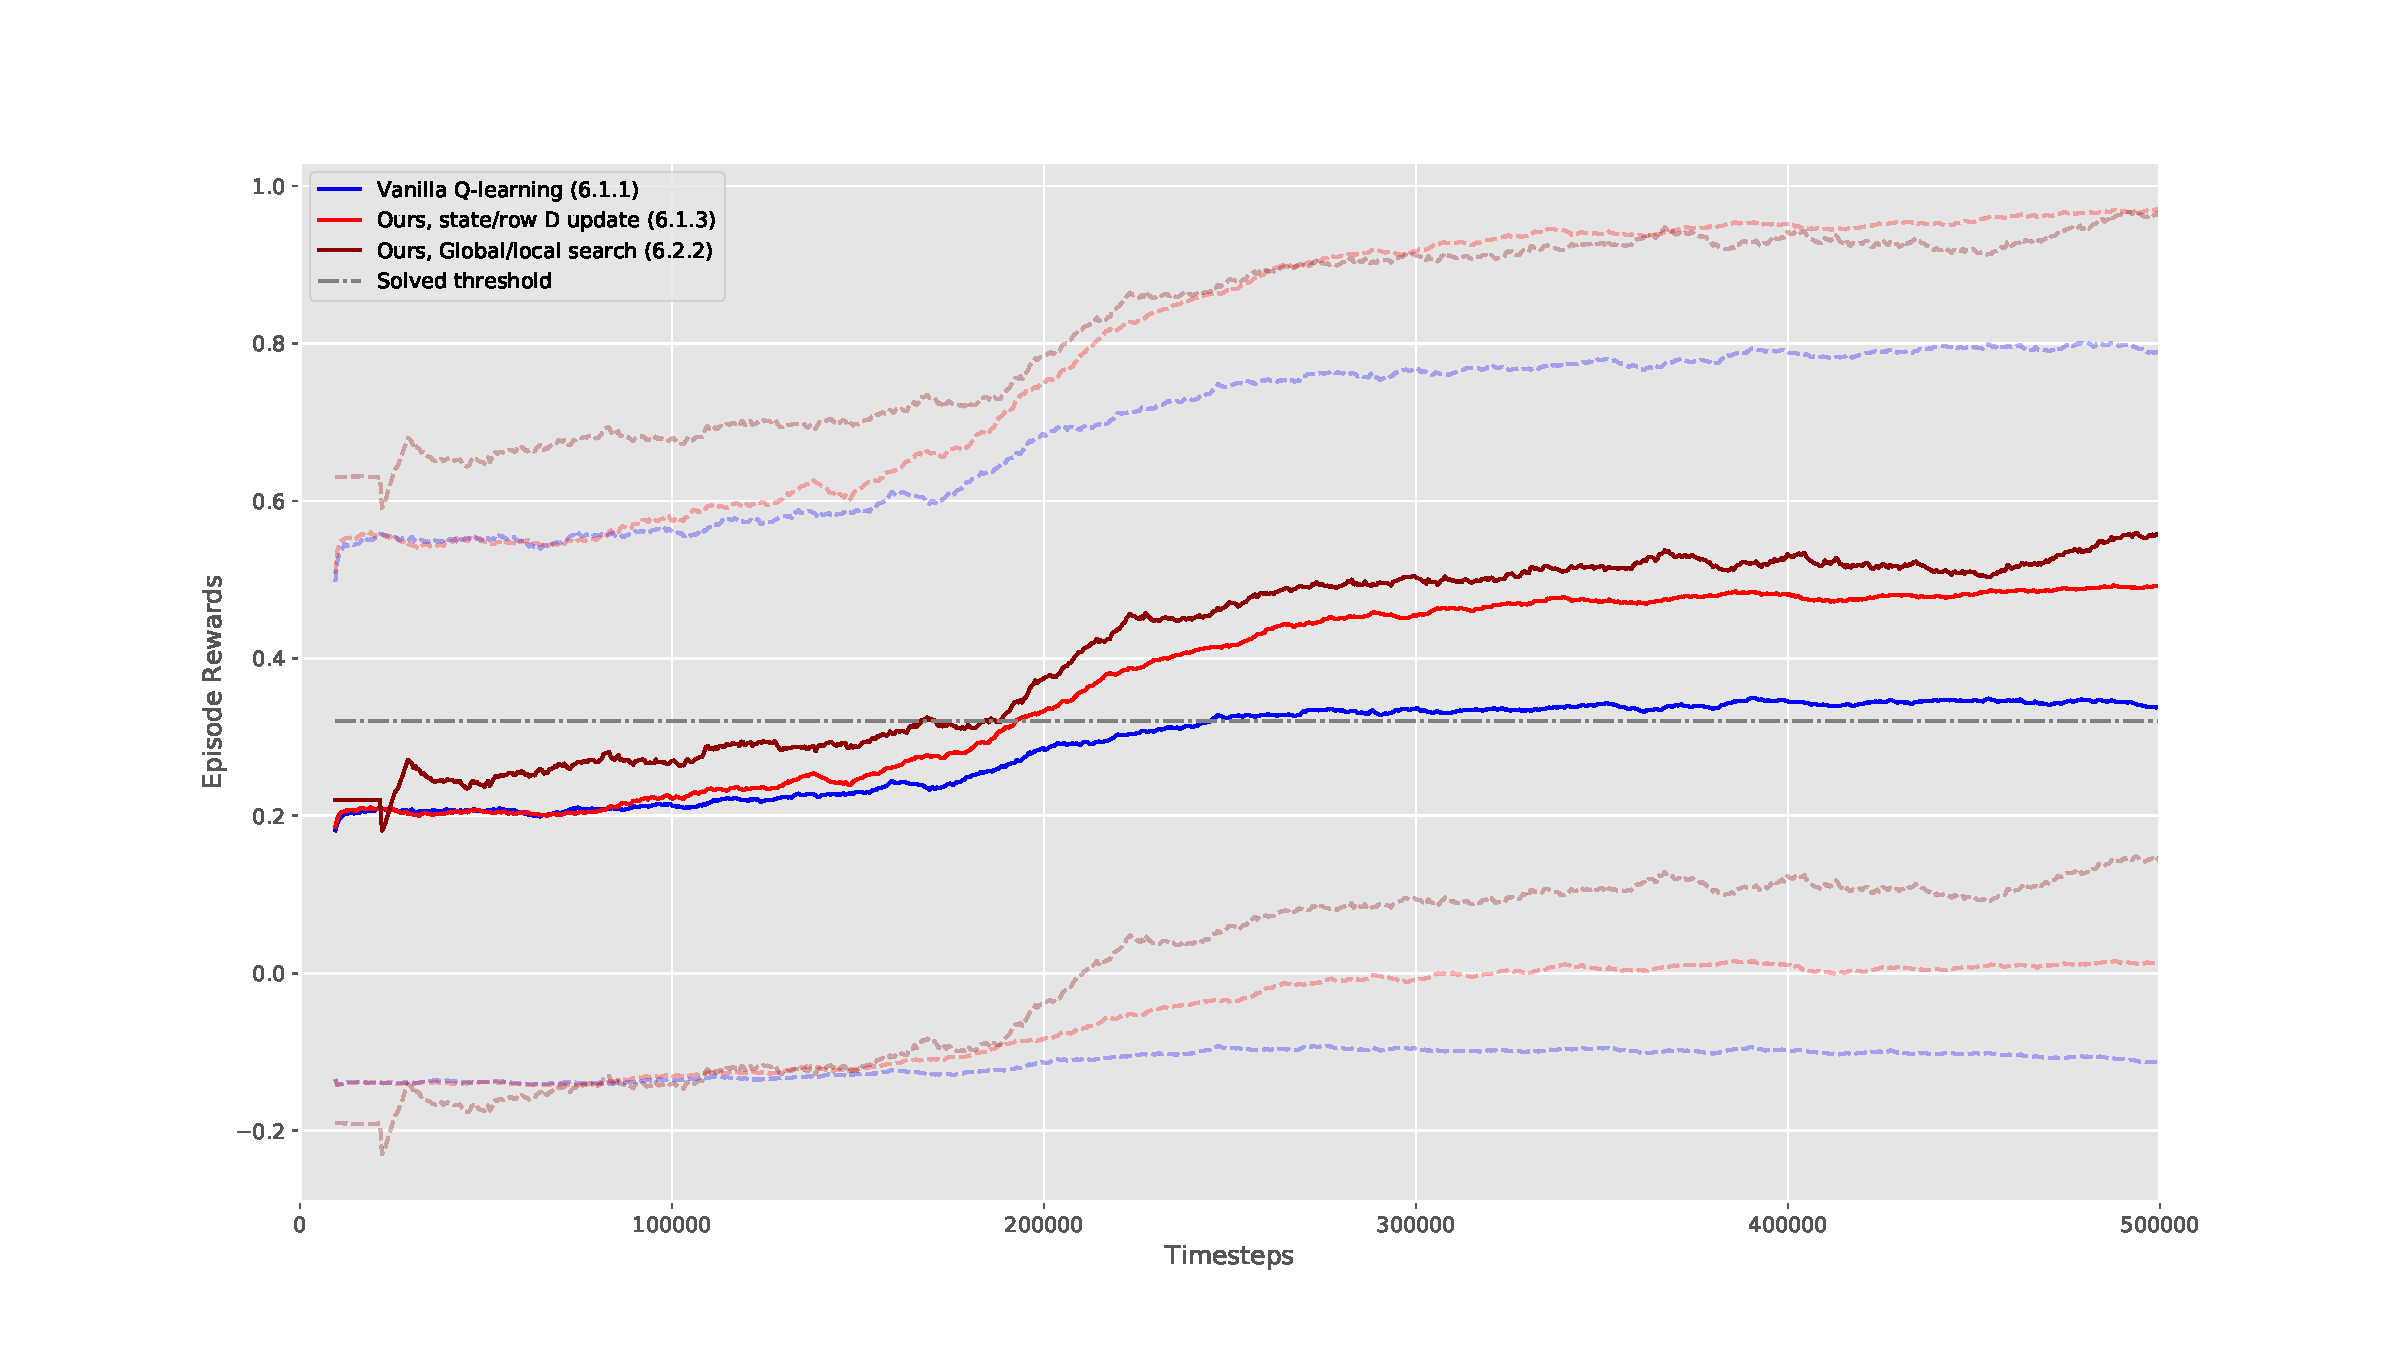
\includegraphics[width=15cm]{Figures/globallocalsearchBench}
\caption{Q-learning with state/action pair update: Rewards over timesteps}
\label{fig:globallocalsearchBench}
\end{figure}

\begin{table}[H]
\centering
\begin{tabular}{@{}ll@{}}
\toprule
Transfer learning approach & AuC     \\ \midrule
Global/local search (approach~\ref{ssec:localglobalsearch})  & 2028.64 \\
Q-table state/pair update (approach~\ref{ssec:QlearningGANPair})  & 1816.29 \\
Vanilla GAN (baseline)     & 1420.80 \\
\end{tabular}
\caption{Area under the curve of different approaches in descending order of AuC}
\label{tab:aucgenerator}
\end{table}
